%%%%%%%%%%%%%%%%%%%%%%%%%%%%%%%%%%%%%%%%%
% Beamer Presentation
% LaTeX Template
% Version 1.0 (10/11/12)
%
% This template has been downloaded from:
% http://www.LaTeXTemplates.com
%
% License:
% CC BY-NC-SA 3.0 (http://creativecommons.org/licenses/by-nc-sa/3.0/)
%
%%%%%%%%%%%%%%%%%%%%%%%%%%%%%%%%%%%%%%%%%

%----------------------------------------------------------------------------------------
%	PACKAGES AND THEMES
%----------------------------------------------------------------------------------------

\documentclass{beamer}

\mode<presentation> {

%\usetheme{default}
%\usetheme{AnnArbor}
%\usetheme{Antibes}
%\usetheme{Bergen}
%\usetheme{Berkeley}
%\usetheme{Berlin}
%\usetheme{Boadilla}
%\usetheme{CambridgeUS}
%\usetheme{Copenhagen}
%\usetheme{Darmstadt}
%\usetheme{Dresden}
%\usetheme{Frankfurt}
%\usetheme{Goettingen}
%\usetheme{Hannover}
%\usetheme{Ilmenau}
%\usetheme{JuanLesPins}
%\usetheme{Luebeck}
\usetheme{Madrid}
%\usetheme{Malmoe}
%\usetheme{Marburg}
%\usetheme{Montpellier}
%\usetheme{PaloAlto}
%\usetheme{Pittsburgh}
%\usetheme{Rochester}
%\usetheme{Singapore}
%\usetheme{Szeged}
%\usetheme{Warsaw}


%\usecolortheme{albatross}
%\usecolortheme{beaver}
%\usecolortheme{beetle}
%\usecolortheme{crane}
%\usecolortheme{dolphin}
%\usecolortheme{dove}
%\usecolortheme{fly}
%\usecolortheme{lily}
%\usecolortheme{orchid}
%\usecolortheme{rose}
%\usecolortheme{seagull}
%\usecolortheme{seahorse}
%\usecolortheme{whale}
%\usecolortheme{wolverine}

%\setbeamertemplate{footline} % To remove the footer line in all slides uncomment this line
%\setbeamertemplate{footline}[page number] % To replace the footer line in all slides with a simple slide count uncomment this line

\setbeamertemplate{navigation symbols}{} % To remove the navigation symbols from the bottom of all slides uncomment this line
}

\usepackage{graphicx} % Allows including images
\usepackage{booktabs} % Allows the use of \toprule, \midrule and \bottomrule in tables
\usepackage{dirtytalk}
\usepackage{tikz}
\usepackage{multicol}
\usepackage{enumerate}
\usepackage{textcomp}

\usetikzlibrary{shapes.geometric, arrows}
\tikzstyle{process} = [rectangle, minimum width=3cm, minimum height=1cm, text centered, draw=black, fill=orange!30]
\tikzstyle{arrow} = [thick,->,>=stealth]

%----------------------------------------------------------------------------------------
%	TITLE PAGE
%----------------------------------------------------------------------------------------

\title[Pi-Casso]{Pi-Casso: A retro LED art platform} % The short title appears at the bottom of every slide, the full title is only on the title page

\author[Group MSB]{}% Your name
\institute[ICL] % Your institution as it will appear on the bottom of every slide, may be shorthand to save space
{
Imperial College London \\ % Your institution for the title page
\medskip
}
\date{June 17, 2016} % Date, can be changed to a custom date

\begin{document}

\begin{frame}
  \vfill
  \centering
  \begin{beamercolorbox}[sep=8pt,center,shadow=true,rounded=true]{title}
    \text{Pi-Casso: A retro LED art platform}\insertsectionhead\par%
  \end{beamercolorbox}
  \vfill
\end{frame}

\begin{frame}
\frametitle{Introduction} 
 
\say{Everything you can imagine is real...}\\
\begin{flushright}
{- \textit{Pablo Picasso }}
\end{flushright}
\text{ }\\
\begin{flushright}
{ \textit{ }}
\end{flushright}
\end{frame}

\begin{frame}
\frametitle{Introduction} 
 
\say{Everything you can imagine is real...}\\
\begin{flushright}
{- \textit{Pablo Picasso }}
\end{flushright}
\say{But only if it fits in 256 LEDs.}\\

\begin{flushright}
{- \textit{Group MSB}}
\end{flushright}

\end{frame}

\begin{frame}
  \vfill
  \centering
  \begin{beamercolorbox}[sep=8pt,center,shadow=true,rounded=true]{title}
    \text{Demo}\insertsectionhead\par%
  \end{beamercolorbox}
  \vfill
\end{frame}


\begin{frame}
\frametitle{Overview} % Table of contents slide, comment this block out to remove it
\tableofcontents % Throughout your presentation, if you choose to use \section{} and \subsection{} commands, these will automatically be printed on this slide as an overview of your presentation
\end{frame}


%------------------------------------------------
%	PRESENTATION SLIDES
%------------------------------------------------

%------------------------------------------------

\section{Design}
\subsection{Inspiration}
\subsection{Deviation}

%------------------------------------------------

\begin{frame}
\frametitle{Design: Inspiration}

\begin{columns}

\begin{column}{0.05\textwidth}
\end{column}

\begin{column}{0.45\textwidth}
\begin{figure}
	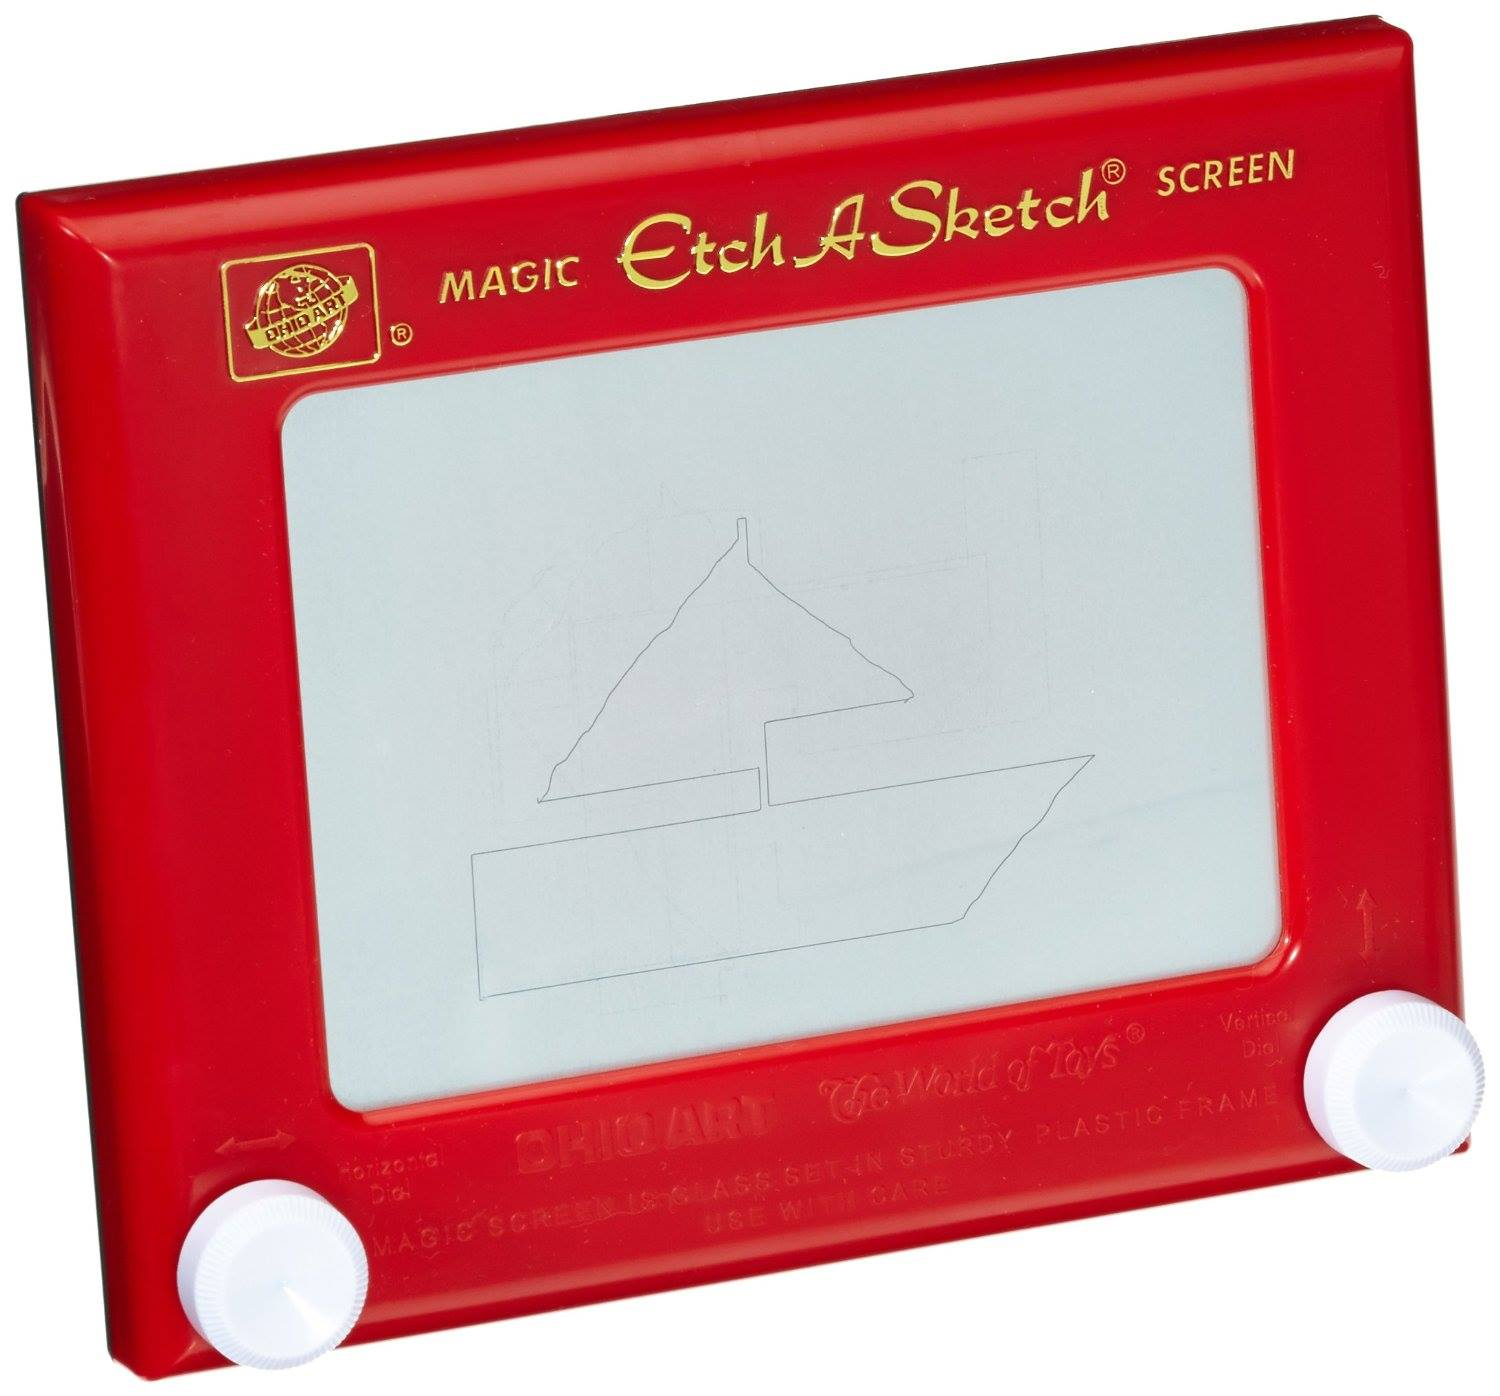
\includegraphics[scale=0.1]{images/etch_a_sketch.jpg}
	\caption{Etch A Sketch}
\end{figure}
\end{column}

\begin{column}{0.45\textwidth}
\begin{center}
\begin{Large}
	\say{Good artists copy. \\Great artists steal.}
\end{Large}
\end{center}
\begin{flushright}
{- \textit{Pablo Picasso }}
\end{flushright}
\end{column}

\begin{column}{0.05\textwidth}
\end{column}

\end{columns}

\end{frame}

%------------------------------------------------

\begin{frame}
\frametitle{Design: Deviation}

\begin{columns}

\begin{column}{0.05\textwidth}
\end{column}

\begin{column}{0.4\textwidth}
Changed:
	\begin{itemize}
	\item Erasing on shaking
	\item Drawing mechanics
	\end{itemize}
Added:
	\begin{itemize}
	\item Animations
	\item Gallery
	\item Pen up/down
	\end{itemize}
\end{column}

\begin{column}{0.5\textwidth}
\begin{figure}
	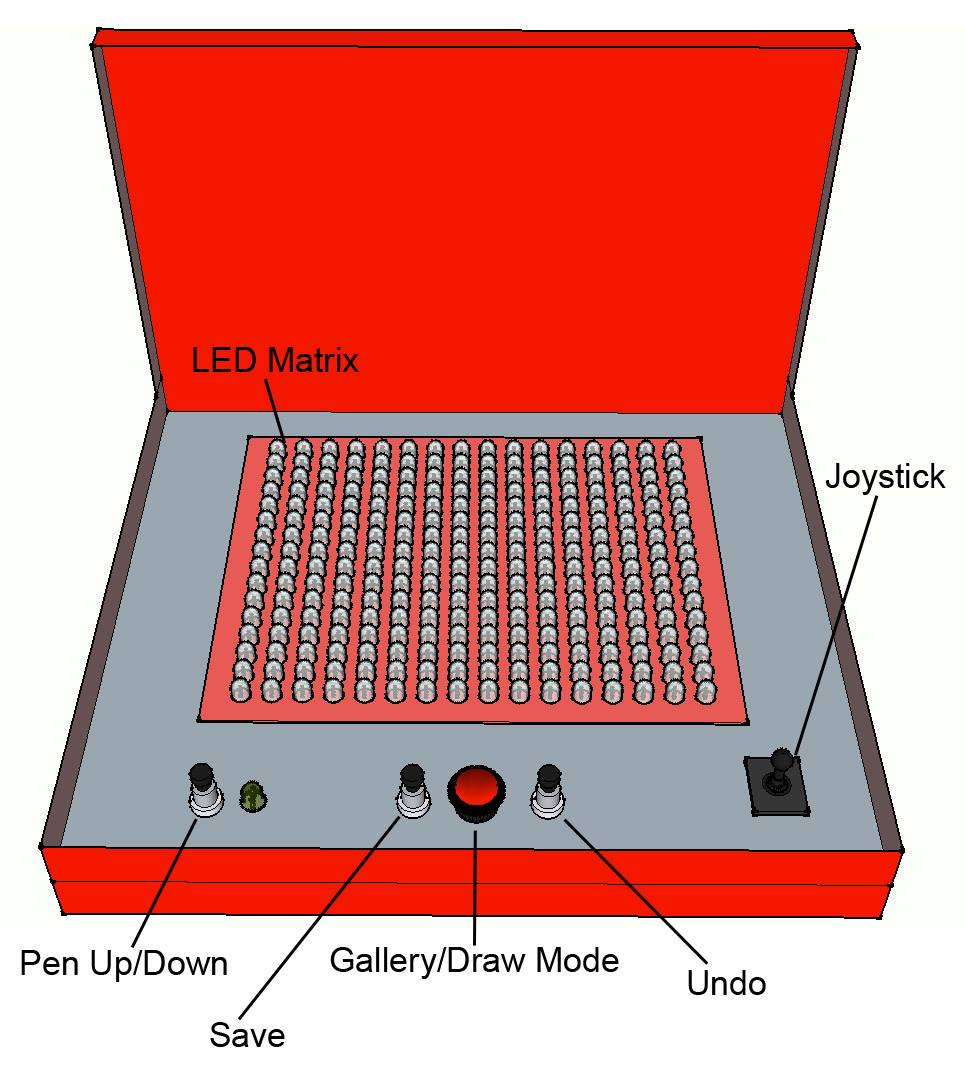
\includegraphics[scale=0.17]{images/sketchup_labels.jpg}
	\caption{Model made in Google SketchUp}
\end{figure}
\end{column}

\begin{column}{0.05\textwidth}
\end{column}

\end{columns}

\end{frame}

%------------------------------------------------
%------------------------------------------------


\section{Development}
\subsection{Hardware}
\subsection{Software}
\subsection{Testing}

%------------------------------------------------
\begin{frame}
\frametitle{Development: Hardware}

\begin{figure}
	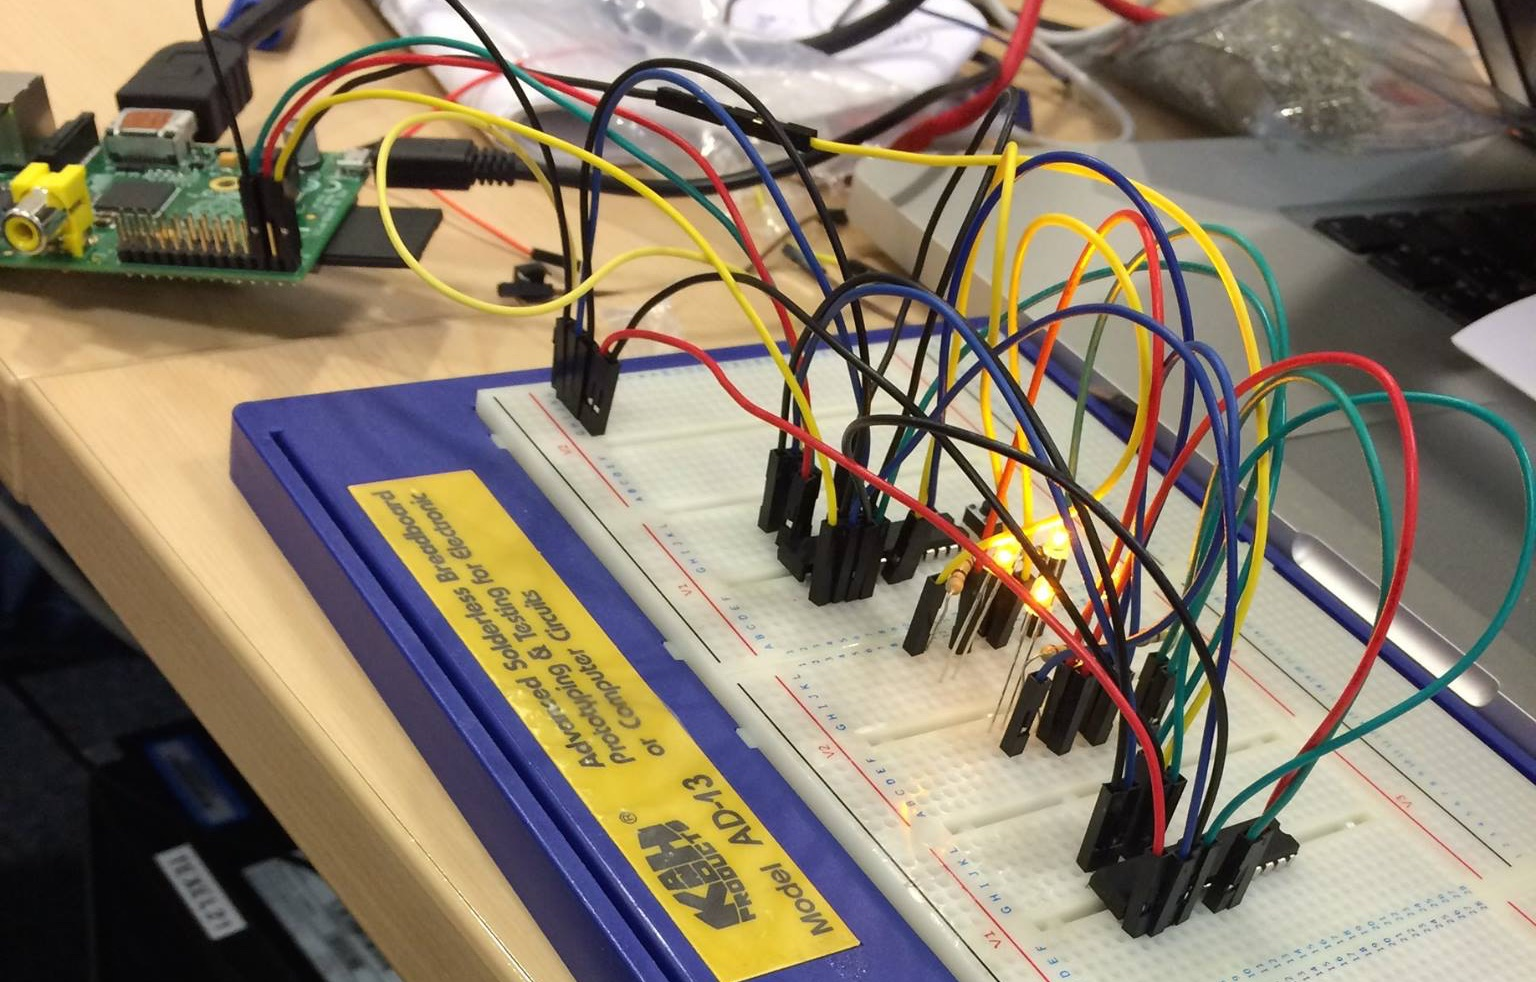
\includegraphics[scale=0.12]{images/matrix_with_resistors.jpg}
	\caption{2x2 LED matrix with resistors}
\end{figure}

\textbf{Solution:} Constantly blink the LEDs (0.1ms ON and 0.9ms OFF).
$$Duty = \frac{Time_{ON}}{Time_{ON} + Time_{OFF}}$$

\end{frame}

%------------------------------------------------
\begin{frame}
\frametitle{Development: Hardware}

\begin{figure}
	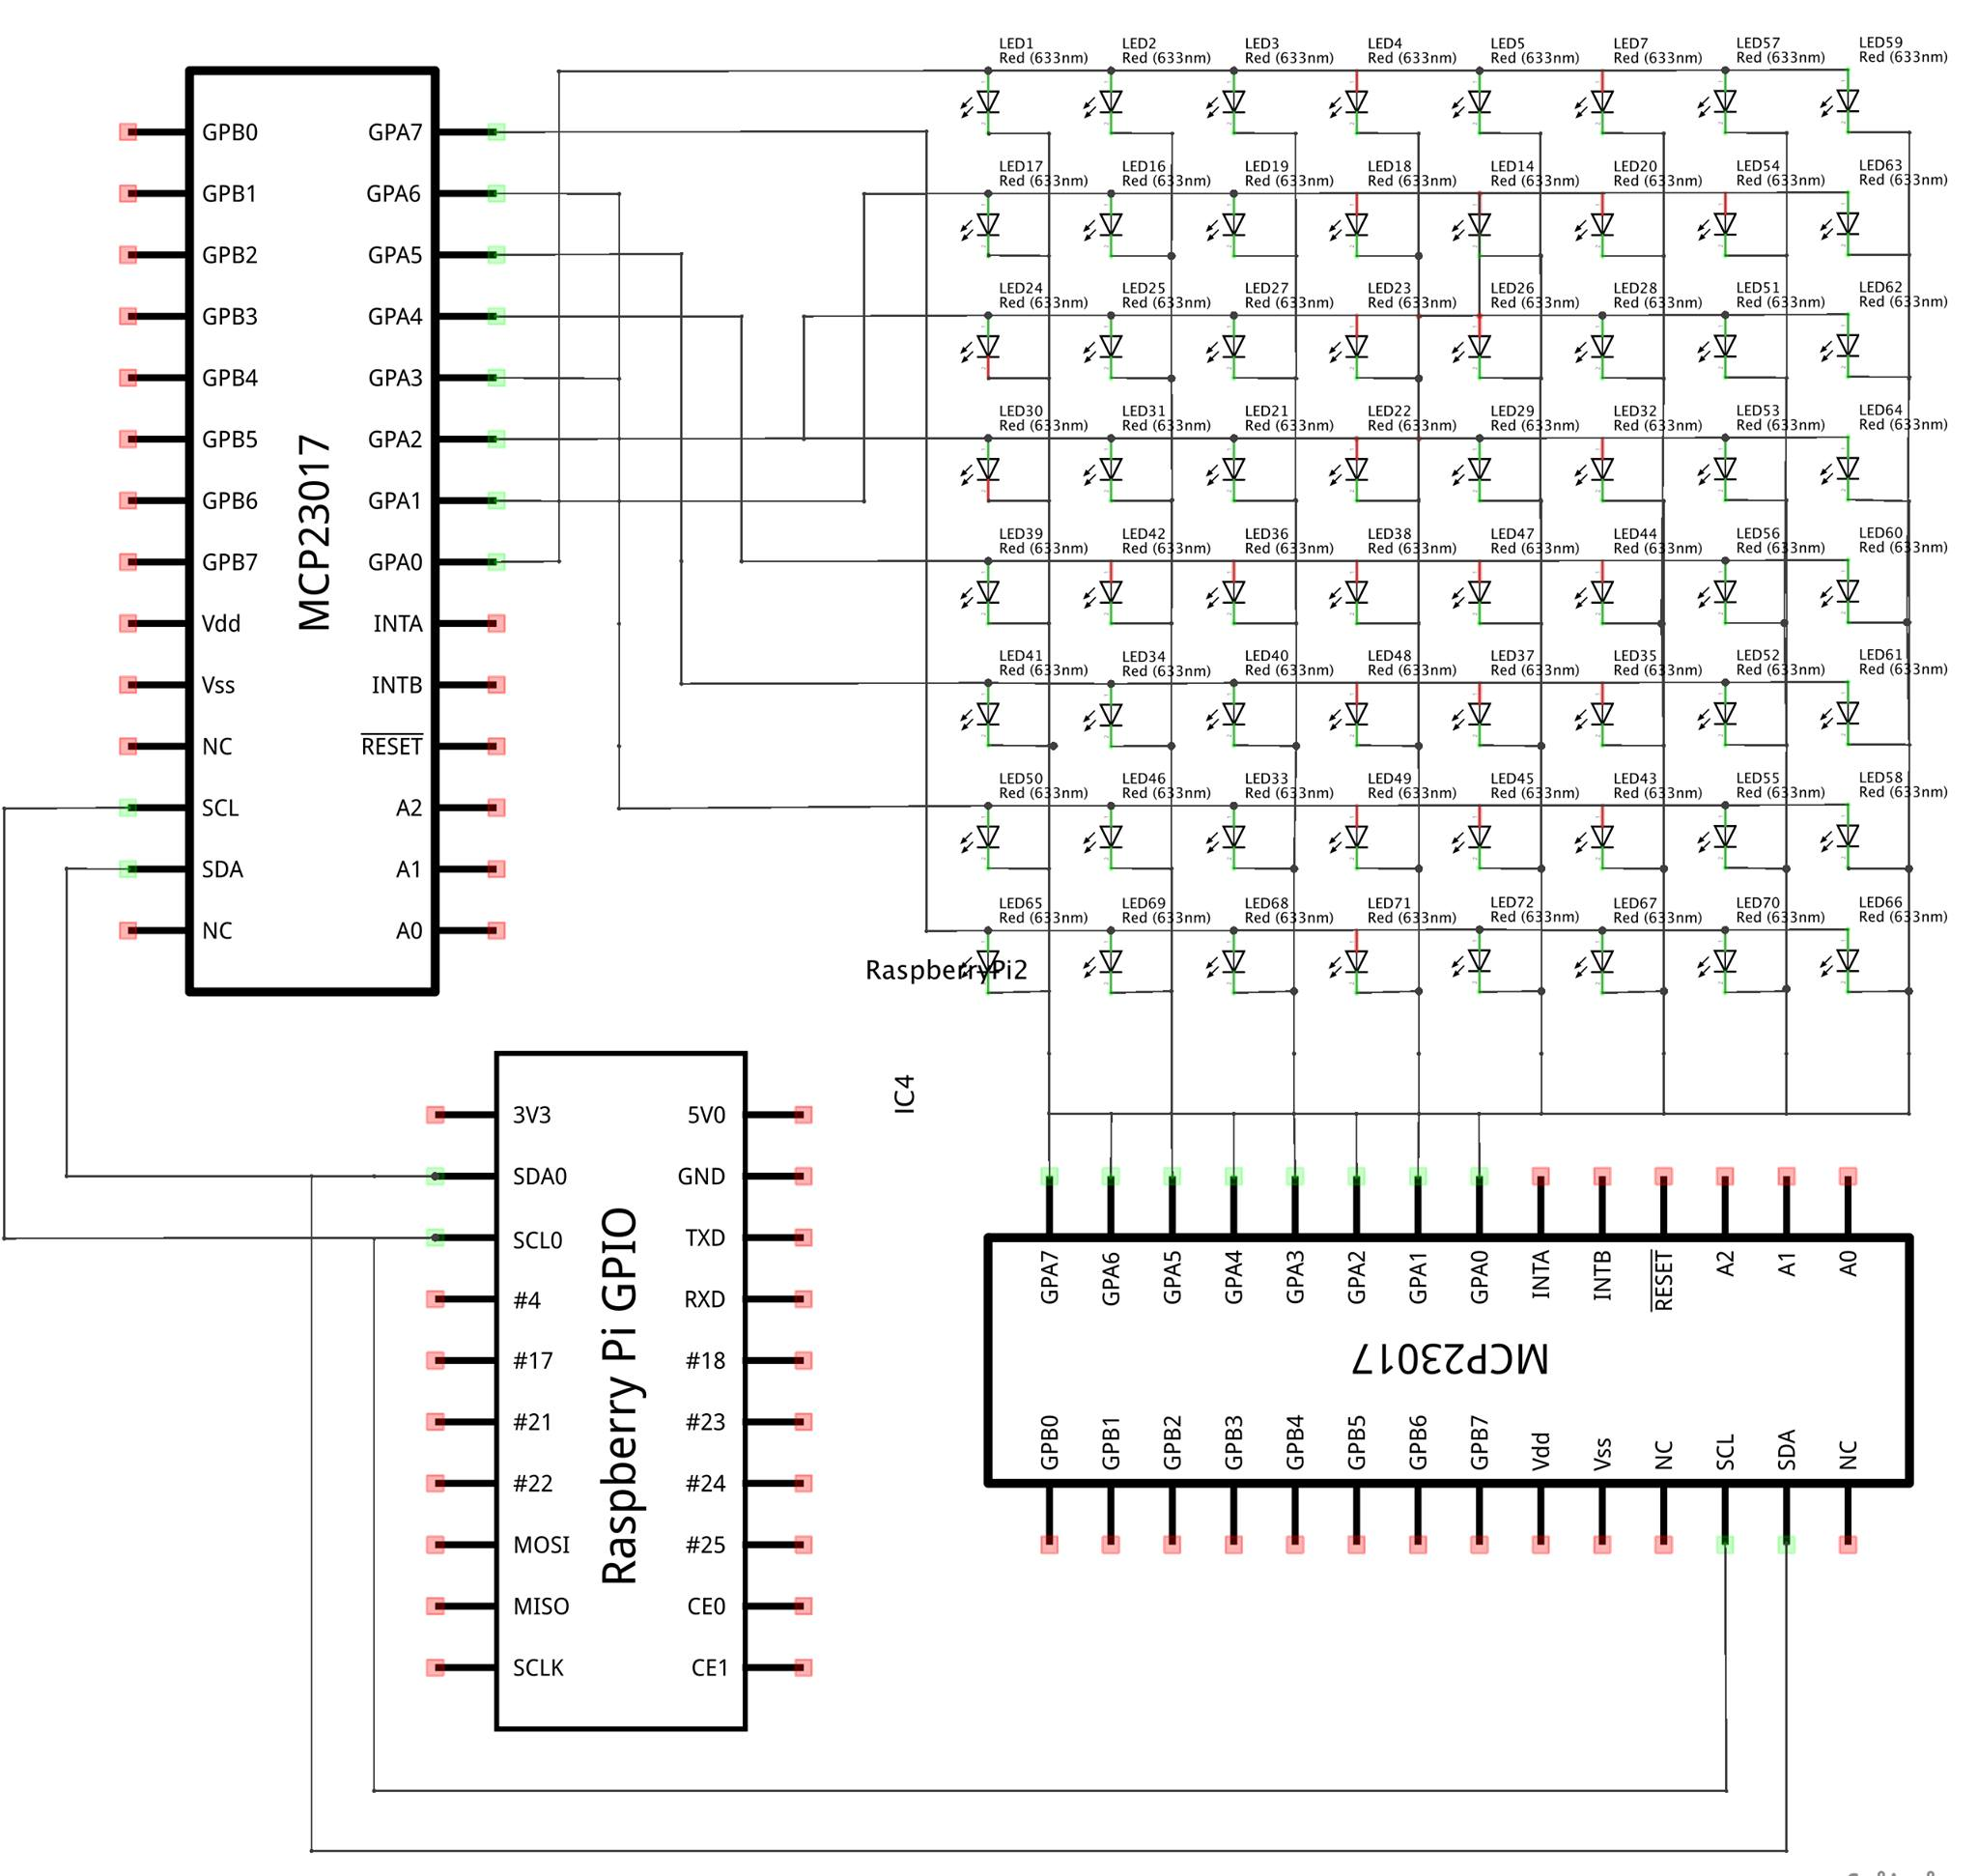
\includegraphics[scale=0.1]{images/circuit_diagram.jpg}
	\caption{Expanding RaspberryPi GPIO using shift registers (MCP23017)}
\end{figure}

\end{frame}

%------------------------------------------------
\begin{frame}[fragile]
\frametitle{Development: Software}

\begin{columns}

\begin{column}{0.025\textwidth}
\end{column}

\begin{column}{0.45\textwidth}
\begin{block}{Image structure}
\begin{verbatim}
typedef struct image
{
  uint32_t rows[SIZE];
  led_t    *last_led; 
} image_t;
\end{verbatim}
\end{block}
\end{column}

\begin{column}{0.05\textwidth}
\end{column}

\begin{column}{0.45\textwidth}
\begin{block}{LED structure}
\begin{verbatim}
typedef struct led
{
  uint8_t x, y;
  uint8_t flash;
} led_t;
\end{verbatim}
\end{block}
\end{column}

\begin{column}{0.025\textwidth}
\end{column}

\end{columns}

\begin{figure}
	\begin{flushleft}
		Example of the information stored in each row:
	\end{flushleft}
	
\includegraphics[scale=0.26]{images/row_example.jpg}
\end{figure}

\end{frame}

%------------------------------------------------
\begin{frame}[fragile]
\frametitle{Development: Software - Display}

\begin{block}{display()}
\begin{verbatim}
for (int i = 0; i < DETECTION_RATE; i++)
{
  gradient_t grad = GRAD_1;
  for (int j = 0; j < 2^(BITS_X_LED) - 1; j++)
  {
    for (int k = 0; k < SIZE; k++)
    {
      switch_on_row(k, rows[k], grad);
      delay(0.1);
      switch_off(k);
    }
    grad++;
  }
} 
\end{verbatim}
\end{block}


\end{frame}

%------------------------------------------------
\begin{frame}
\frametitle{Development: Software - Detect}

\begin{figure}
	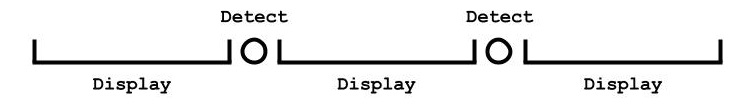
\includegraphics[scale=0.3]{images/detect_display.jpg}
	\caption{Detect/display cycle intervals}
\end{figure}

In {\tt detect()} the input from the buttons is read and the image is changed according to the current mode:
\begin{itemize}
	\item Draw
	\item Move
	\item Gallery
\end{itemize}

\end{frame}

%------------------------------------------------
\begin{frame}
\frametitle{Development: Software - Step I }

\begin{figure}
	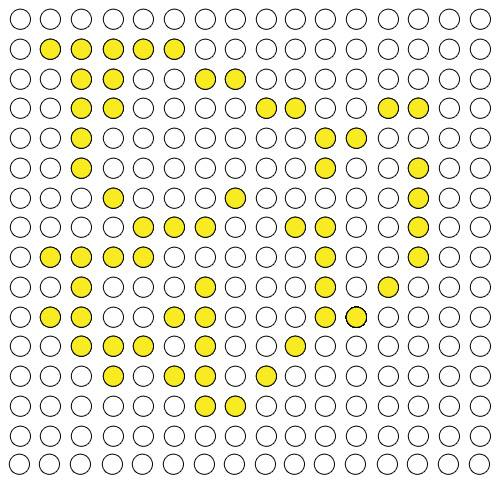
\includegraphics[scale=0.4]{images/example_1.jpg}
	\caption{Initial image}
\end{figure}

\end{frame}

%------------------------------------------------
\begin{frame}
\frametitle{Development: Software - Draw}

\begin{enumerate}
\item Displacement is detected
\item If pen is down, {\tt last\_led} is switched on
\item If the destination position is in bounds, {\tt last\_led} is moved accordingly
\end{enumerate}

\end{frame}

%------------------------------------------------
\begin{frame}
\frametitle{Development: Software - Step II }

\begin{figure}
	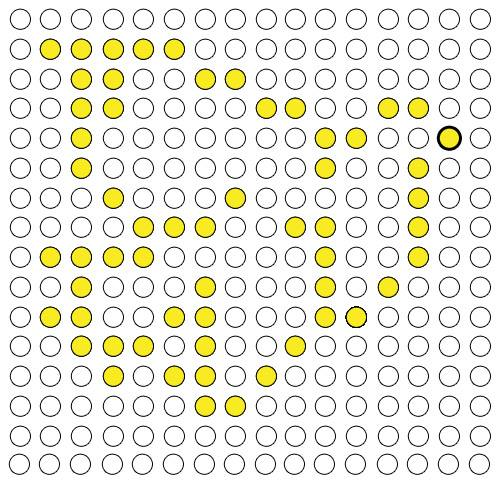
\includegraphics[scale=0.4]{images/example_2.jpg}
	\caption{Image after drawing LED in position (15, 5)}
\end{figure}

\end{frame}

%------------------------------------------------
\begin{frame}
\frametitle{Development: Software - Move}

\begin{columns}

\begin{column}{0.05\textwidth}
\end{column}

\begin{column}{0.45\textwidth}
\begin{figure}
	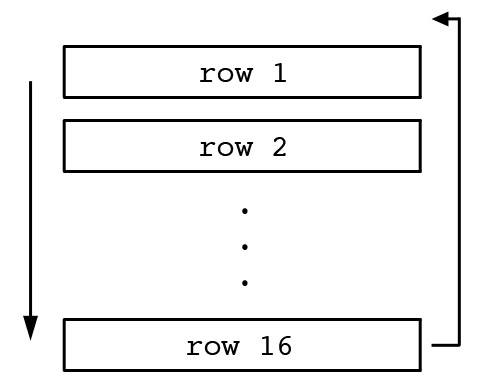
\includegraphics[scale=0.22]{images/vertical_rotation.jpg}
	\caption{Vertical rotation (down)}
\end{figure}
\end{column}

\begin{column}{0.45\textwidth}
\begin{figure}
	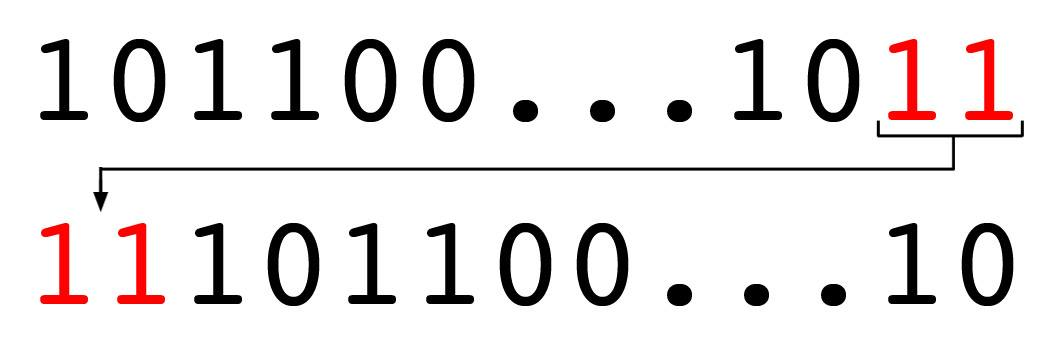
\includegraphics[scale=0.14]{images/horizontal_rotation.jpg}
	\caption{Horizontal rotation (right)}
\end{figure}
\end{column}

\begin{column}{0.05\textwidth}
\end{column}

\end{columns}

{\tt move} acts as a buffer between {\tt draw} and {\tt gallery}:
\begin{itemize}
\item It fetches the previously drawn image and stores it
\item Keeps track of all the moves for posterior reproduction in the gallery
\end{itemize}

\end{frame}

%------------------------------------------------
\begin{frame}
\frametitle{Development: Software - Step III}

\begin{figure}
	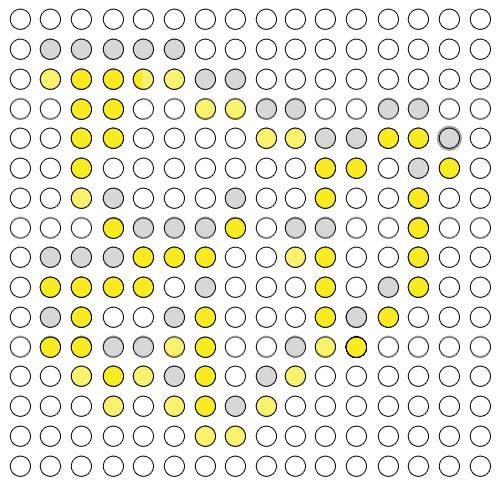
\includegraphics[scale=0.4]{images/example_3.jpg}
	\caption{Image moved down 1 row}
\end{figure}

\end{frame}

%------------------------------------------------
\begin{frame}
\frametitle{Development: Software - Step IV}

\begin{figure}
	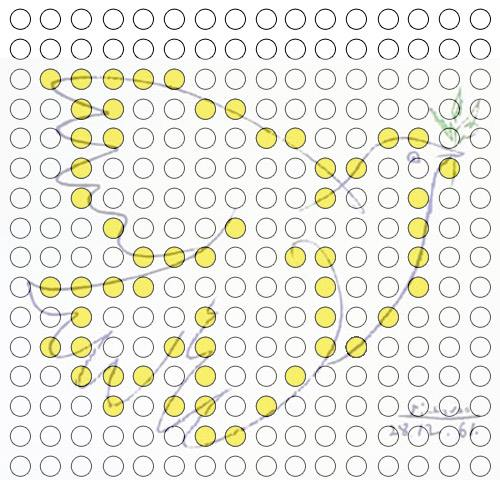
\includegraphics[scale=0.4]{images/example_final.jpg}
	\caption{Can you tell what it is yet?}
\end{figure}

\end{frame}

%------------------------------------------------
\begin{frame}
\frametitle{Development: Software - Gallery}

{\tt gallery\_control} contains the access procedures of a doubly linked list used both to:
\begin{itemize}
	\item Navigate through your saved images/videos
	\item Loop through the frames of each video
\end{itemize}

{\tt gallery} takes advantadge of it using iterators

\end{frame}

%------------------------------------------------

\begin{frame}
\frametitle{Development: Testing}

\begin{columns}

\begin{column}{0.05\textwidth}
\end{column}

\begin{column}{0.4\textwidth}
\begin{figure}
	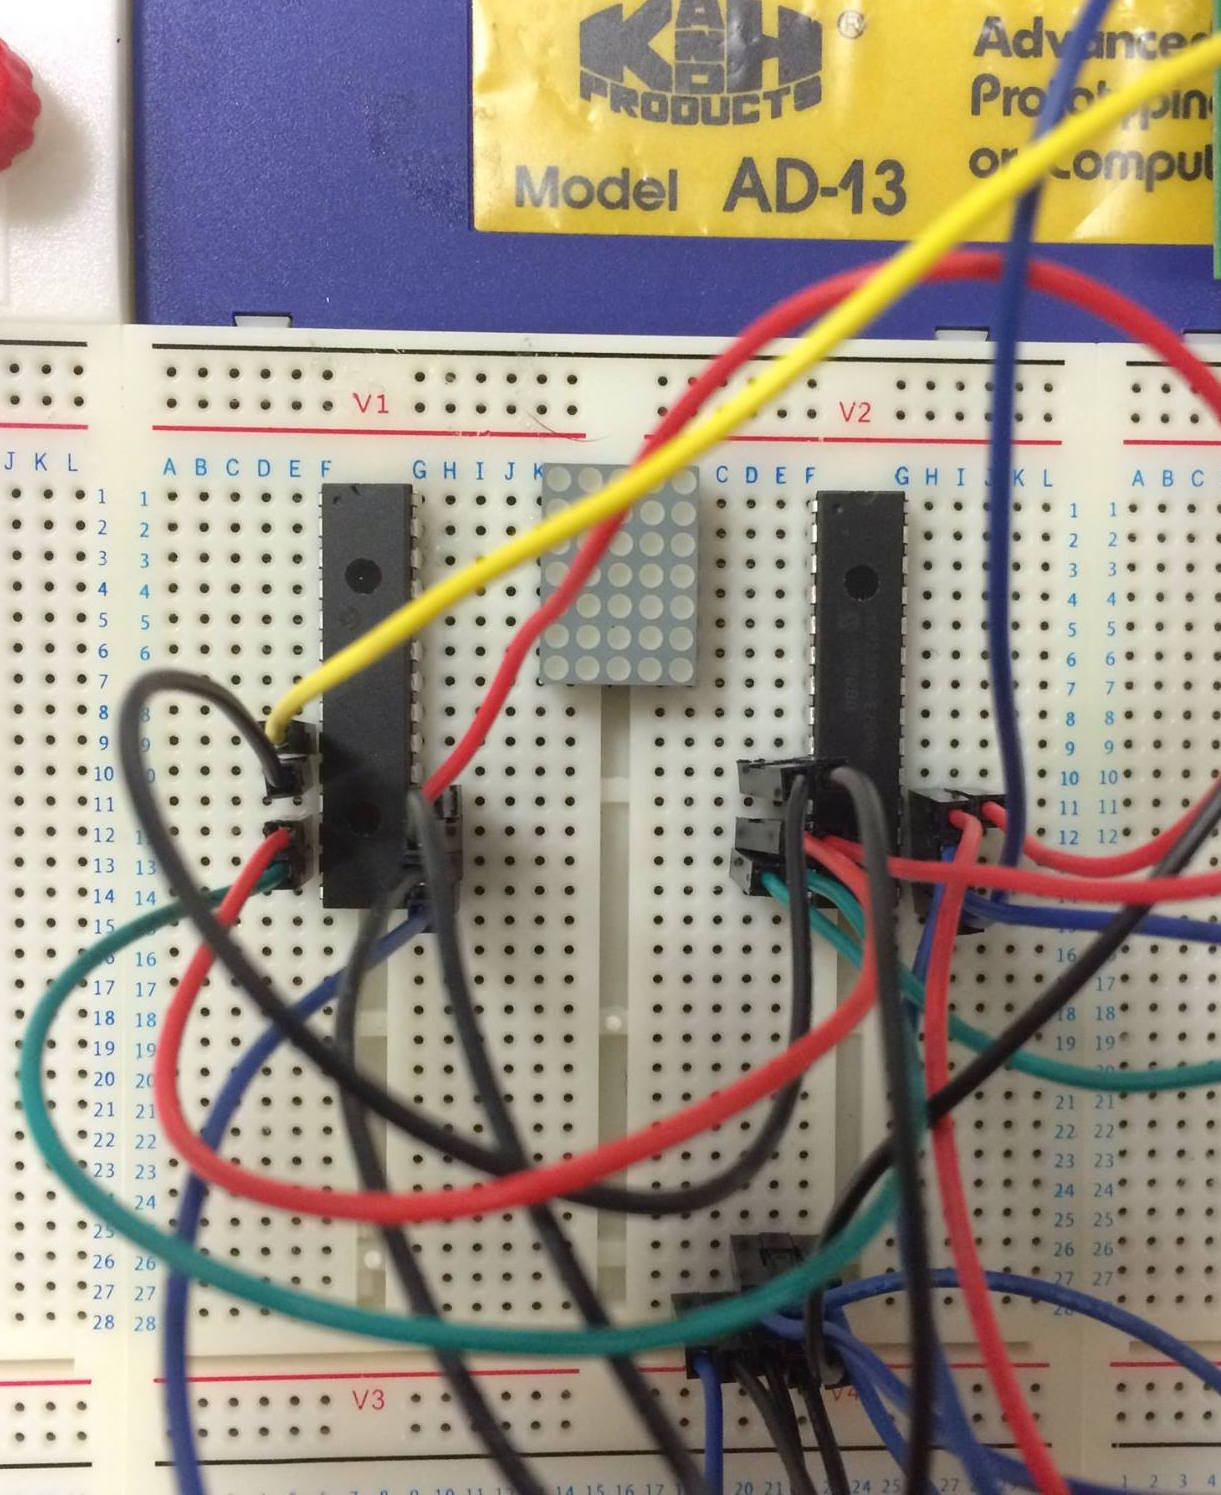
\includegraphics[scale=0.1]{images/led_matrix.jpg}
	\caption{5x7 pre-made matrix}
\end{figure}
\end{column}


\begin{column}{0.4\textwidth}
\begin{figure}
	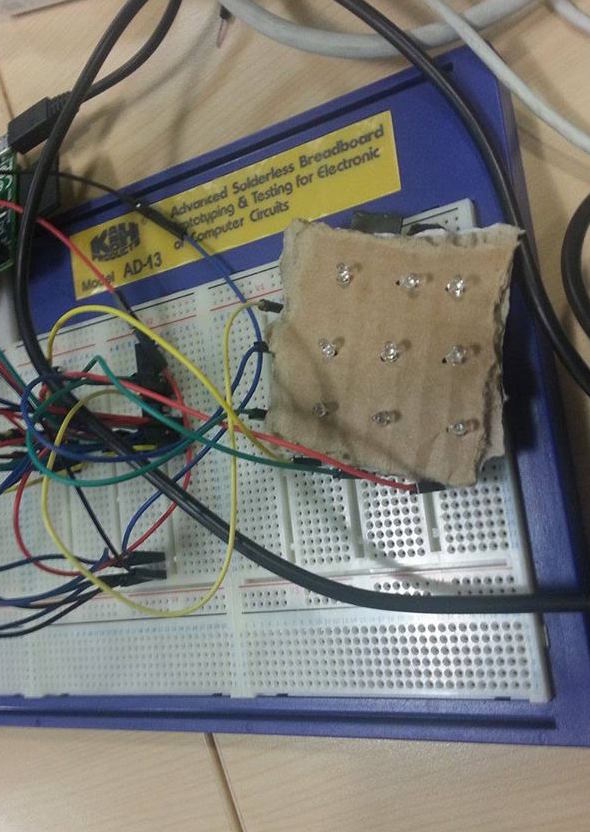
\includegraphics[scale=0.181]{images/cardboard_matrix.jpg}
	\caption{3x3 prototype on card}
\end{figure}
\end{column}

\begin{column}{0.05\textwidth}
\end{column}

\end{columns}

\end{frame}

%------------------------------------------------

\begin{frame}
\frametitle{Development: Testing}

Once in the EEE robotics lab:
\begin{itemize}
\item \say{Switching one LED at a time won't work!} - Adam Heywood
\item Issues with the electronics
\end{itemize}

\begin{columns}

\begin{column}{0.05\textwidth}
\end{column}

\begin{column}{0.4\textwidth}
\begin{figure}
	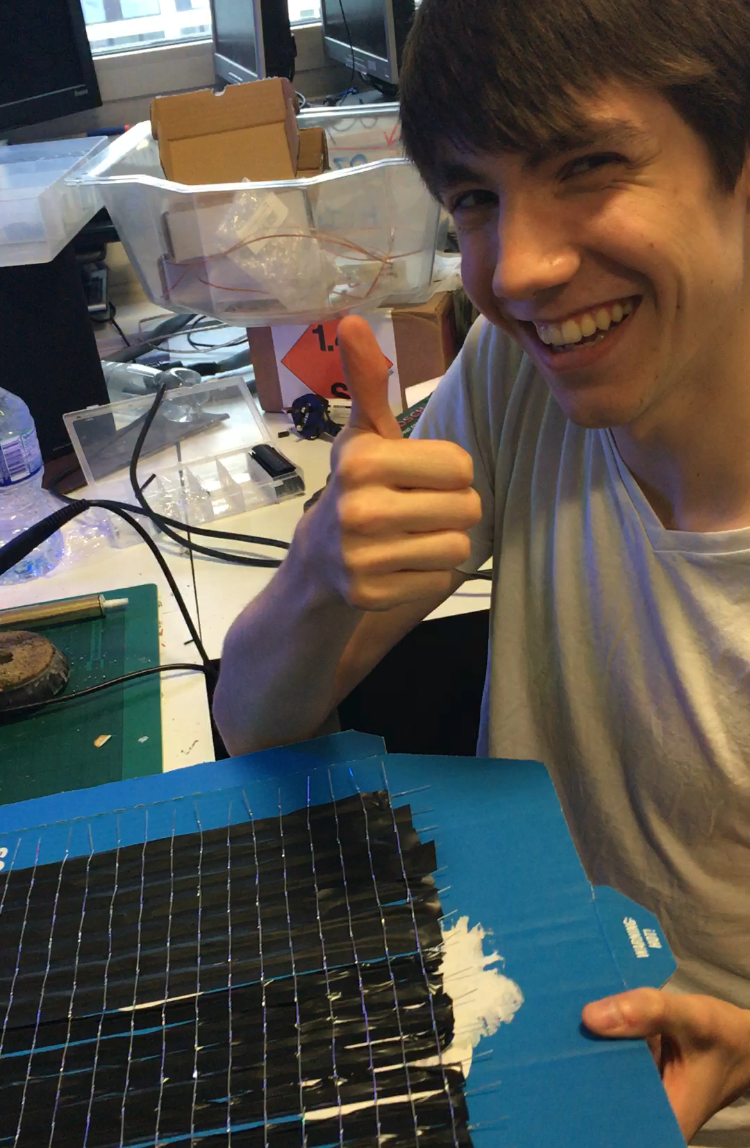
\includegraphics[scale=0.1]{images/bad_connections.png}
	\caption{LED matrix with bad connections}
\end{figure}
\end{column}


\begin{column}{0.4\textwidth}
\begin{figure}
	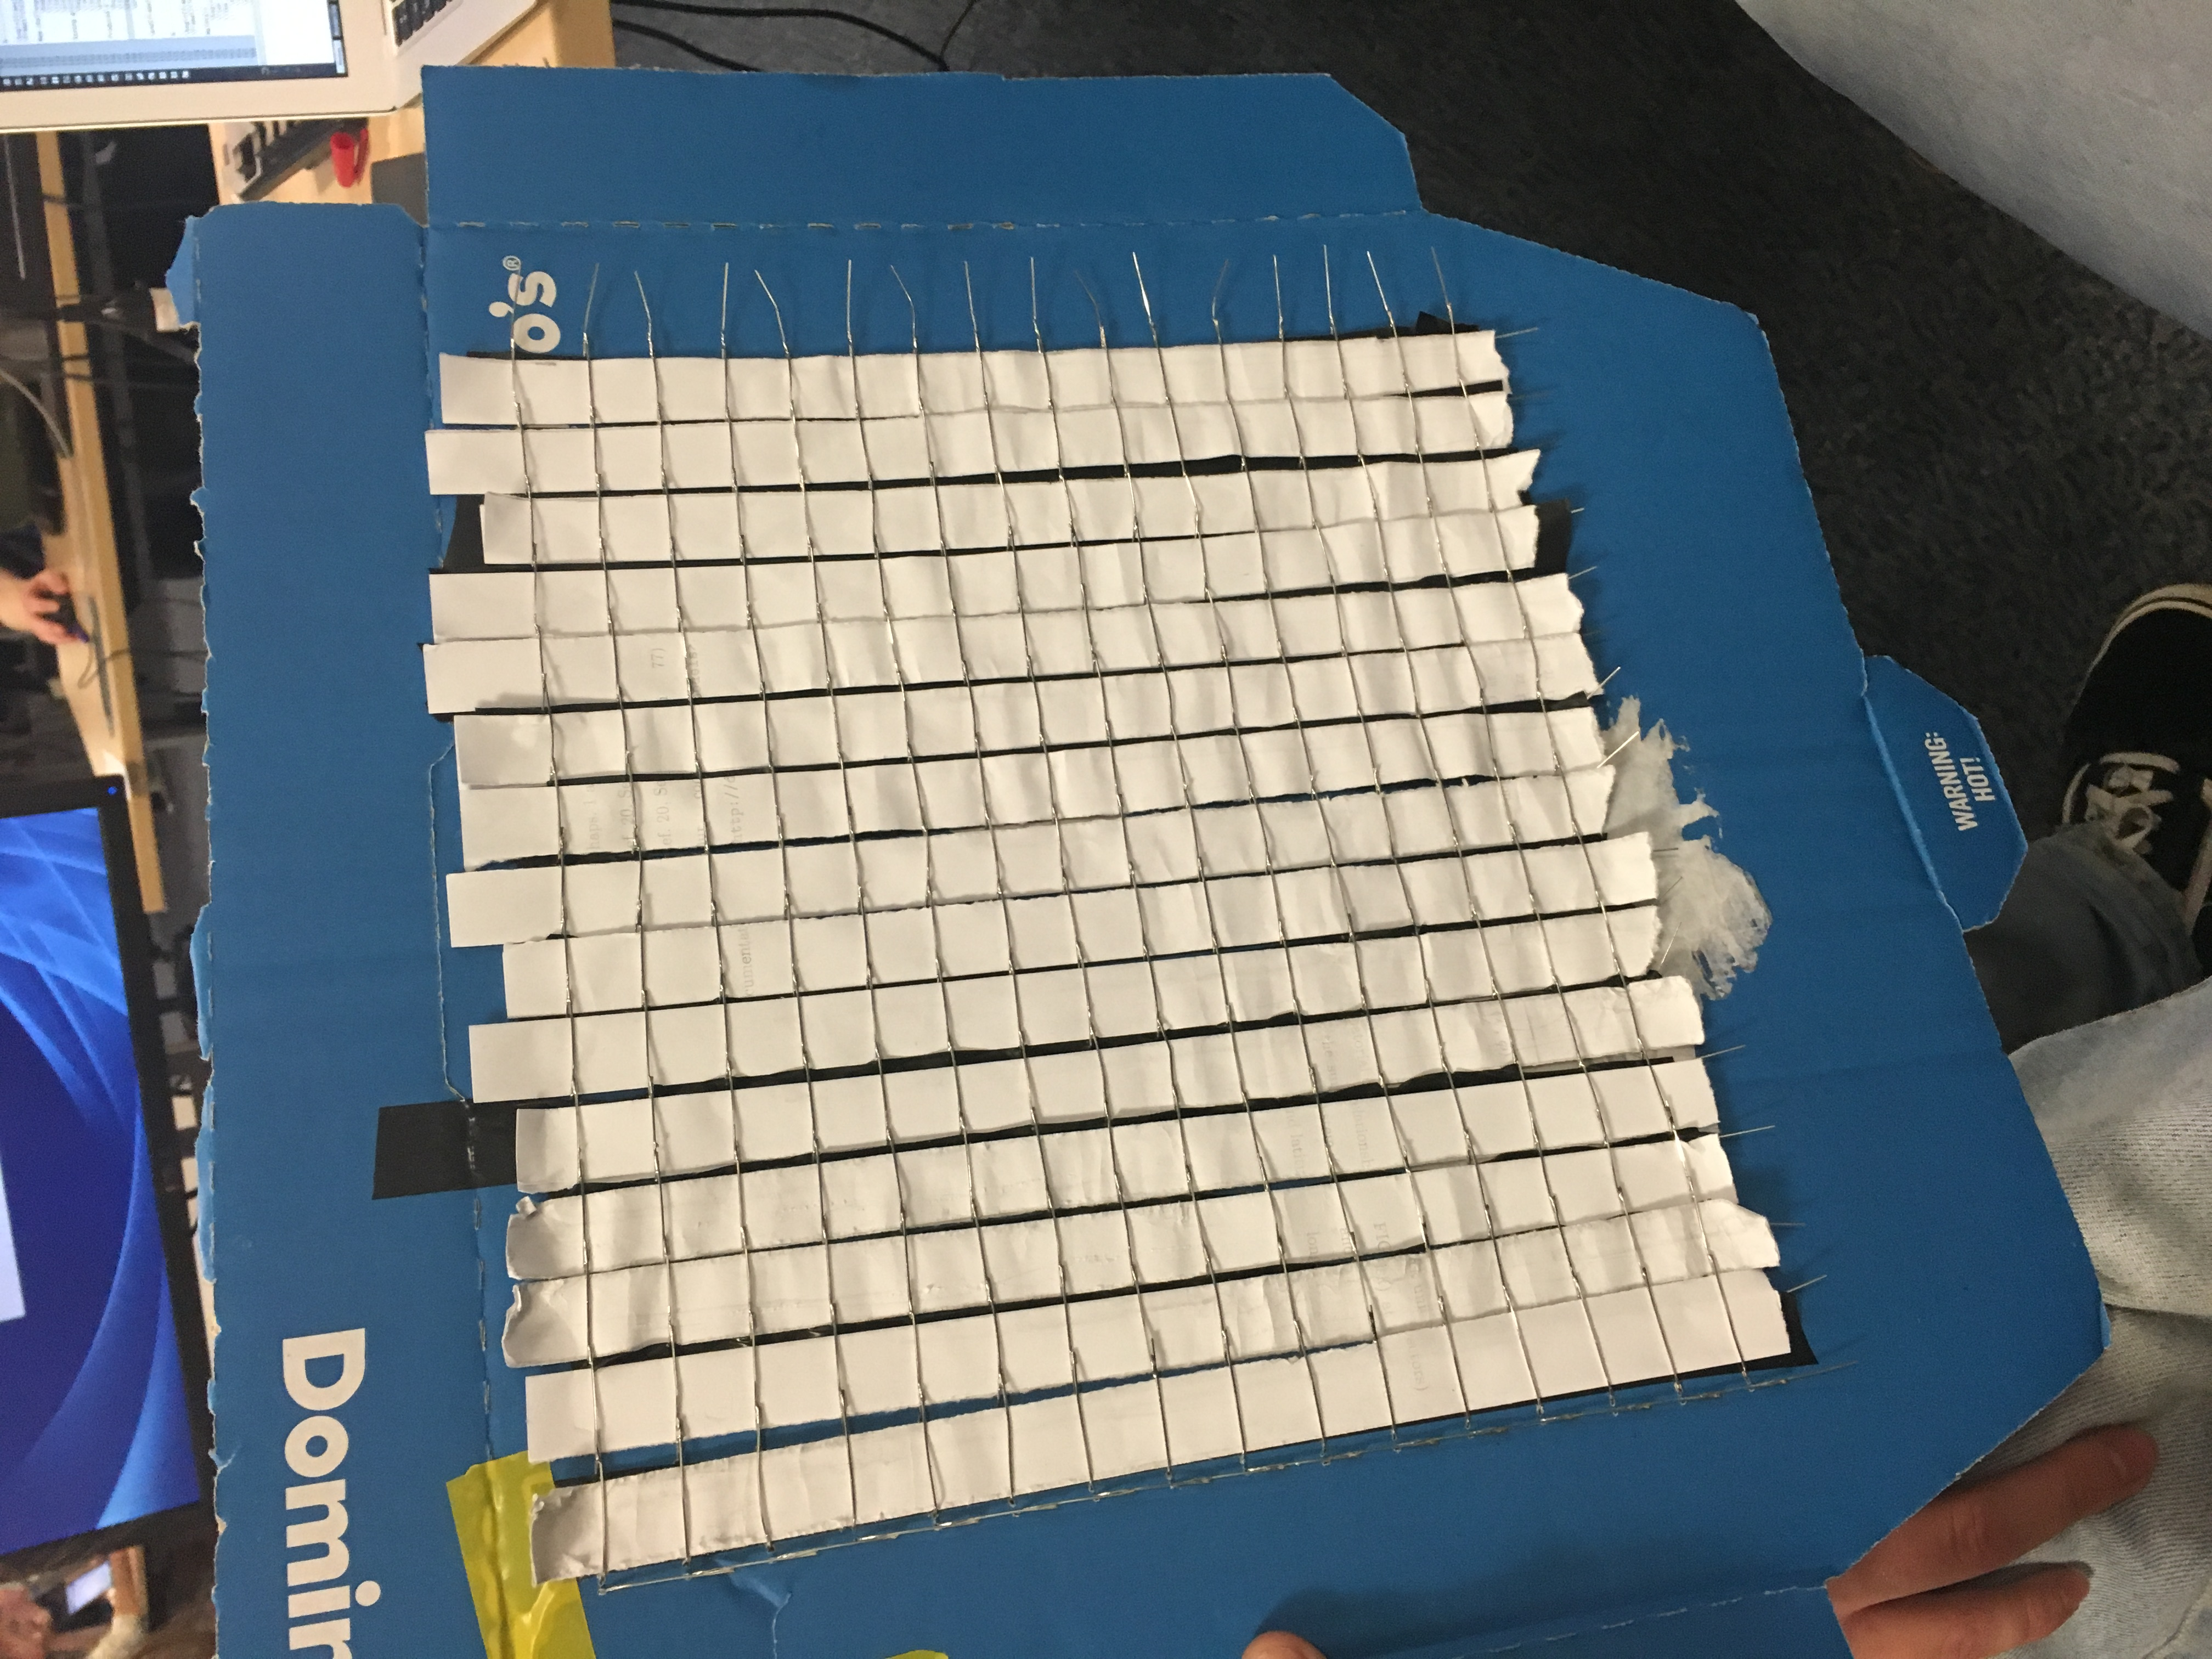
\includegraphics[scale=0.032]{images/good_connections.jpg}
	\caption{LED matrix with paper fix}
\end{figure}
\end{column}

\begin{column}{0.05\textwidth}
\end{column}

\end{columns}

\end{frame}


%------------------------------------------------
%------------------------------------------------

\section{Reflection}
\subsection{What went well}
\subsection{If we were to do it again}

%------------------------------------------------

\begin{frame}
\frametitle{Reflection: What went well}

New challenges
		\begin{itemize}
		\item Learning C 'on the fly'
		\item Implementing electronics
		\end{itemize}
Strong group dynamic
		\begin{itemize}
		\item Perseverance and rigorousness in problem solving
		\item Communication of ideas and issues
		\end{itemize}
Produced a tangible product
		\begin{itemize}
		\item Originality of approach
		\item Ambitious use of hardware
		\end{itemize}

\end{frame} 	


%------------------------------------------------

\begin{frame}
\frametitle{Reflection: If we were to do it again}

Maintain:
	\begin{itemize}
	\item Planning conceptually first
	\item Communication
		\begin{itemize}
		\item Awareness of what others are doing
		\end{itemize}
	\end{itemize}
Change:
	\begin{itemize}
	\item Use of {\tt git}
	\item Time management
		\begin{itemize}
		\item Planning use of materials
		\item Restructure entire code
		\item Earlier testing
		\end{itemize}
	\end{itemize}

\end{frame}

%------------------------------------------------

\begin{frame}
\Huge{\centerline{Any questions?}}
\end{frame}

%----------------------------------------------------------------------------------------

\end{document} 